\documentclass[a4paper]{report}
\usepackage{graphicx}
\usepackage{epsfig}
\usepackage{latexsym}
\usepackage{url}
\begin{document}

\title{Initial Report}
\author{Oasis Team}

\maketitle



\section*{1 Project Description }
\subsection* {1.1 Project Overview}
Our team’s aim is making a file synchronization tool, which contains both desktop and mobile clients to download and upload files across multiple devices. Dropbox will be the blueprint of this project, and we will try to add some features to our version. After a few discussions in the first week, we decided to divide our team into three sub-team, which are front-end, server, and mobile respectively.  Since our team members have different backgrounds and strengths, we thought it would be better to divide them into the right place.  

\subsection* {1.2 Project Architecture}
In order to implement the Android application and web application for this project, we design the software architecture as Figure 1. HTTP protocol will be used both for Android application and web application to download and upload files. For the Android application, its design and implementation will follow the Material Design. For the web application, Bootstrap and Angular will be used for front-end development, and Spring MVC will be applied to back-end development, Hibernate will be used as a persistent tool for the MySQL database.



\begin{figure}[h]
\centering
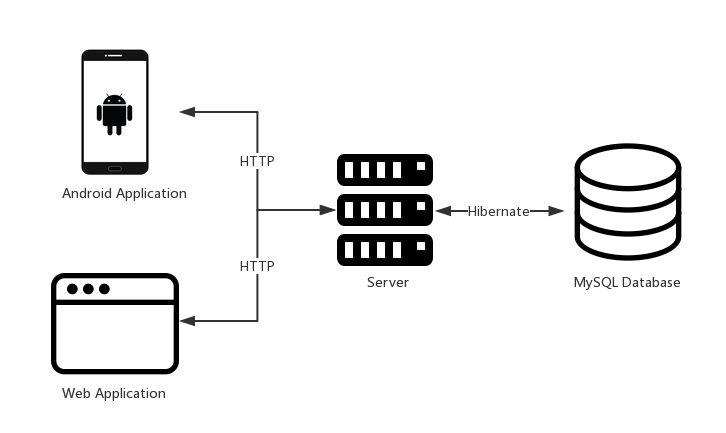
\includegraphics[width=4.6in]{figure1}
\end{figure}

\subsection* {1.3 Project Methodology}
We choose agile development as our development methodology. Agile development takes the evolution of user's needs as the core, and it uses an iterative, step-by-step approach to software development. Scrum is a framework for developing and maintaining complex products and is an incremental, iterative development process. In this framework, the entire development process consists of several short iteration cycles, a short iteration cycle called a Sprint. We use it to control the process of our development.


Tehao Ye is the product owner of our product. He is mainly responsible for determining the function of the product and meeting the required standards, specifying the release date and delivery content of the software.Yibo Liu is the scrum master. She is mainly responsible for the smooth implementation of the entire Scrum process in the project. At the same time,she should ensure the communication among the team member and the development work.All of the members in our group constitute the development team. The development team is mainly responsible for the development of software products under the Scrum process. Each member is responsible for different technical aspects. Members can work in any way as long as they can achieve Sprint's goals.


\subsection* {1.4  Project Timetable }

As for the rough timetable, our level 1 will focus on the primary function of our software such as uploading and downloading files for both desktop and mobile users.  Before moving to level 2, we hope that our software would meet the basic requirements for a synchronization tool. As for level 2, our main idea is adding some key features to our project, and one of the essential features is making sure the synchronize method works well. At the end of this semester, we will test and make user manual for our project.




\begin{figure}[h]
\centering
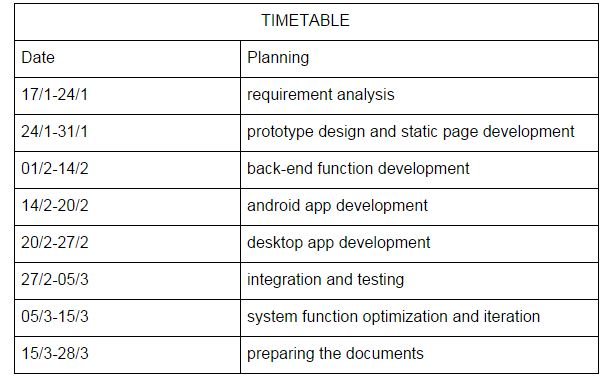
\includegraphics[width=4.6in]{1}
\end{figure}

\section* {2 Project Organization}
\subsection* {2.1 How you will work together as a group}

We have divided our group into two parts: Android app and the Desktop app.
Android App: Tehao Ye and Yankai Chen are responsible for the development of the Android app. Their tasks are designing the prototype and technical development. 
Desktop App: Yibo Liu, Mohan Chi, and Jiawei Ding are responsible for the prototype designing, and front-end development. Zhihao Zhu and Jiawei Zhou are responsible for the software architecture and server development.


\begin{figure}[h]
\centering
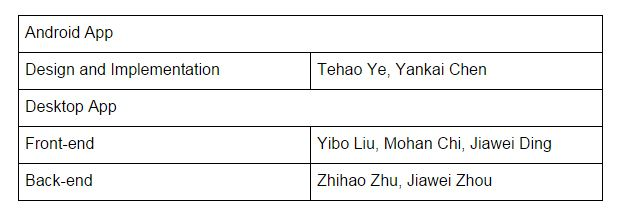
\includegraphics[width=4.6in]{2}
\end{figure}

\subsection* {2.2 The process you expect to use for handling peer assessment
}
Our method for peer assessment is that each member have a primary point at the beginning, and we will add points based on their devotion to this project. Since this is a group project, we hope everyone in our team will be a part of this project. In the other way, we will deduct some points for members, who may not meet the requirements or fail to finish his/her job, and the points will add to other members based on their performance.
\subsection* {2.3 You have agreed upon for handling any conflicts within the team that may arise.
}
We will hold a team meeting once some conflicts occur, and team members will talk through all conflicts. After that, we will vote for different options and make a solution that all members will agree on that. At the worst case, we will talk to the professor in order to get some advice, and we will make the final solution based on those devices.
















	












\end{document}
